\documentclass[12pt, a4paper]{article}
\usepackage[T1]{fontenc}
\usepackage[utf8]{inputenc}
\usepackage[french]{babel}
\usepackage{geometry}
\usepackage{graphicx}
\usepackage{wrapfig}
\usepackage{indentfirst}
\usepackage{tikz}
\usepackage{igo}
\usepackage{amsfonts}

\graphicspath{{/home/pgi/TIPE/content/Rapport/image/}}
\usetikzlibrary{trees}

% Title
\title{Rapport de TIPE\\
Morpion}
\author{Peng-Wei Chen, MP, \oldstylenums{2017}-\oldstylenums{2018}}
\date{}

\begin{document}

\maketitle
\tikzstyle{point}=[circle,draw,thin,fill=white]

\subsection*{Avant-propos}
Le morpion est un jeu très connu dans le monde dont la stratégie gagnante a été trouvée dans les années 90. Or, on ne sait pas encore si une stratégie gagnante existe lorsque la taille de la grille varie. L'objectif de ce TIPE est de déterminer les tailles de la grille où le premier joueur a une stratégie gagnante.

\section{Introduction}
\subsection{La règle du morpion}
Deux joueurs jouent sur une grille de taille $15 \times 15$ sur le papier. Chacun prend un symbole et on dessine au tour par tour son symbole sur la grille. Le but est d'aligner 5 symboles verticalement, horizontalement ou en diagonale pour gagner.
Dans le cas généralisé, nous appelons (m, n, k)-jeu où la taille de la grille est $m \times n$ et il faut $k$ symboles dans une ligne pour gagner.

\subsection{Méthode}
Il existe deux méthodes pour déterminer s'il existe une telle stratégie:
\begin{itemize}
    \item On cherche tous les cas possibles.
    \item On apparie les points de la grille. Si le deuxième joueur peut toujours prévenir la réussite du premier joueur en jouant le pairage, alors une telle stratégie n'existe pas.
\end{itemize}

Dans le cas où k $\le$ 7, on utilise la première méthode avec l'arbre de décision. Chaque nœud de cet arbre est un état de la grille. Par exemple (\mbox{Figure. \ref{fig:arbre}}) , la racine de cet arbre est la grille sans symbole. Ensuite, les fils de chaque nœud sont les états de la grille où on place un symbole de plus au dessus. Enfin, les feuilles sont les cas où un des joueurs a gagné ou où personne n'a gagné (c'est-à-dire que la grille a été remplie et que aucun joueur n'a aligné k symboles).


Or, la complexité de chercher tous les cas possibles est en O(($m \times n$)!). Ainsi, on utilise une fonction gloutonne pour chercher le cas le \og plus \fg possible. Avec cette fonction, on donne une note à chaque point. Si un point est plus possible pour gagner, alors sa note est plus élevée.\par
On utilise la deuxième méthode lorsque k > 7.

\section{Exploitation}
\subsection{k $\le$ 5}
Afin de diminuer la complexité, on essaie de créer une fonction qui a l'état de la grille comme entrée et renvoie dix positions: ce sont les positions possibles pour gagner. Ainsi, à chaque nœud de l'arbre de décision, on a diminué le nombre de cas possibles de tous les positions à dix positions.
\subsubsection{Fonction naïve}
L'idée est simple: on considère le nombre de symboles non séparés dans une ligne. 
Pour chaque point sur la grille non occupé par les symboles, on définit la \og note \fg \ à valeur dans $\mathbb{N}$ en ce point. La note est caculée selon les quatre directions, dépend du nombre de symbole du premier joueur (On n'utilise cette fonction que pour le premier joueur). Précisément, il y a trois cas possibles. Pour les deux premiers cas, on appelle i-vivant ou i-mort (\mbox{Figure. \ref{fig:vivmort}}) où i est le nombre de symboles déjà aligné, vivant si les deux cotés sont libres, mort si seul un des deux coté est libre. On donne $3^{i}$ au cas de i-vivant et $3^{i-1}$ au celui de i-mort car i-mort est en effet le cas de (i$+$1)-vivant. En particulier, on donne $3^{k+1}$ au cas où le premier joueur est sûrement gagné, c'est-à-dire k-mort ou (k-1)-vivant. Tenant compte des quatre directions, il y a des autres cas autre que k-mort ou (k-1)-vivant que le premier joueur gagne sûrement. Par exemple (Figure. \ref{fig:directions}), si k $=$ 5, le cas 4-mort-4-mort est un cas gagnant (le deuxième joueur ne peut que prévenir la réussite d'une direction, les deux x). Dans le troisième cas, les deux cotés ne sont pas libres, alors on donne 0 selon cette direction (impossible de compléter en k symboles dans la même ligne). La \og note \fg \ est la somme de ces valeurs selon les quatre directions. Par exemple (\box{Figure. \ref{fig:note}}), au point A, on somme 81 ($3^{4}$, horizontale) et $3\times 3$ ($3^1$,verticale et les deux directions diagonales). La note au point A vaut 90.\par

On a ainsi une fonction naïve.

\subsubsection{Améliorer notre fonction avec l'élagage alpha-beta}
Dans notre fonction, on ne considère que le nombre de symboles dans une ligne et elle n'est pas correcte dans certains cas. Par exemple (\mbox{Figure. \ref{fig:besoin}.1}), au début du jeu, le premier joueur place son symbole au centre de la grille. Ensuite, le deuxième joueur place en haut à gauche du centre. Dans ce cas-là, la fonction renvoie 4 positions (\ref{fig:besoin}.2) avec la même note. Cependant, l'une de ces positions donne l'avantage au deuxième joueur. (\ref{fig:besoin}.3) Dans ce cas-là, le deuxième joueur peut défendre et essayer d'aligner ses symboles en même temps. 
\par
On utilise l'arbre de décision pour améliorer notre fonction, de sorte que notre fonction \og pense\fg \ à l'étape d'après. Pour le faire, on utilise l'algorithme de minimax. Dans cet algorithme, on utilise notre fonction naïve et la note est calculée par la difference de celle du premier joueur et celle du deuxième joueur. Cette note peut être eventuellement négative. Ainsi (\mbox{Figure. \ref{fig:minimax}}), dans le niveau du premier joueur (niveau max), on veux que la note soit plus élevée tandis que la note est plus faible dans le niveau du deuxième joueur (niveau min).

%alpha-beta
Dans l'arbre de décision, on donne la note de la position si c'est une feuille. Lorsqu'on est dans un nœud du niveau max (resp. min), on compare les notes de ses fils et en choisit la plus grande (resp. petite). En pratique, on se donne une hauteur et on fait un parcours en profondeur.\par
On peut encore améliorer cet algorithme en utilisant l'algorithme de l'élagage alpha-beta. Dans l'algorithme de minimax, on peut couper les arêtes dans certains cas. Par exemple (\mbox{Figure. \ref{fig:alpha-beta}}), dans le niveau max, on a déjà déterminé la note d'un nœud 81. Or dans le nœud A, sa note est donnée par le minimum du niveau prochain. Ainsi, dans le niveau prochain, on peut s'arrêter dès qu'on a une note inférieure à 81. On appelle coupure alpha (resp. coupure beta) lorsqu'on est dans le niveau max (resp. niveau min) et une des notes des fils d'un nœud est inférieure (resp. supérieure) à celle de son frère.\par
On utilise la fonction améliorée pour chercher la stratégie gagnante du premier joueur.

\subsection{k $\ge$ 8}
On peut montrer que le premier joueur n'a pas de stratégie gagnante lorsque k~=~8, et donc le premier joueur n'en a pas pour tout k $\ge$ 8 car la réussite du (m, n, k)-jeu où k $\ge$ 8 implique la réussite du (m, n, 8)-jeu. On donne notamment la preuve du cas k = 9 \mbox{(Figure. \ref{fig:m-n-9})} car il est plus intuitif.
On voit que si le deuxième joueur suit le pairage, alors le premier joueur ne peut jamais réussir (les lignes rouges).\newpage
Lorsque k = 8, on divise le jeu en des sous-jeux. Ces sous-jeux se jouent sur la grille de la forme comme \mbox{Figure. \ref{fig:sous-jeu}.}
Il y a trois façons de gagner ce sous-jeu \mbox{(Figure. \ref{fig:regle}):}
\begin{itemize}
    \item Aligner trois symboles en diagonale.
    \item Aligner verticalement deux symboles.
    \item Aligner horizontalement quatre symboles.
\end{itemize}
Ainsi, puisque le premièr joueur ne peut jamais gagner ce sous-jeu, il ne peut pas non plus gagner le (m, n, 8)-jeu. (Figure. \ref{fig:m-n-8})
\section{Conclusion}

\begin{itemize}
    \item k = 3
    \item k = 4
    \item k = 5
    \item k $\ge$ 8\\
        Une telle stratégie n'existe pas.
\end{itemize}

\section{Annexe}

%% Figure: arbre de decision
\begin{figure}[h]
    \centering
    \gobansize{3}
    \black{b2}
    \copytogoban{2}
    \white{a3}
    \copytogoban{3}
    \clear{a3}
    \white{a2}
    \copytogoban{4}
    \cleargoban
    \black{a2}
    \copytogoban{5}
    \clear{a2}
    \black{a3}
    \copytogoban{6}
    \clear{a3}

\begin{tikzpicture}[level distance=2cm,
    level 1/.style={sibling distance=4cm},
level 2/.style={sibling distance=1.5cm}]
  \node {\showfullgoban}
  child {node {\usegoban{2} \showfullgoban}
      child {node {\usegoban{3} \showfullgoban}
      child {node {$\vdots$}}}
      child {node {\usegoban{4} \showfullgoban}
      child {node {$\vdots$}}}
    }
    child {node {\usegoban{5} \showfullgoban}
        child {node {$\vdots$}}
        child {node {$\vdots$}}
    }
    child {node {\usegoban{6} \showfullgoban}
        child {node {$\vdots$}}
        child {node {$\vdots$}}
    };
\end{tikzpicture}
    \caption{Arbre de décision (le cercle noir est le symbole du premier joueur)} \label{fig:arbre}
\end{figure}

\gobansize{10}
\cleargoban

%% Exemple: 3-vivant, 3-mort
\begin{figure}[h]
    \centering
        \black{d5,e5,f5}
        \shortstack{\showgoban\\3-vivant}
        \white{g5}
        \shortstack{\showgoban\\3-mort}
    \\
    \ \\
        \white{c5}
        \clear{e5}
        \gobansymbol{e5}{A}
        \shortstack{\showgoban\\La note au point A est nulle pour le noir.}
    \caption{3-vivant et 3-mort}
    \label{fig:vivmort}
\end{figure}

\cleargoban
%% Exemple: 2 directions
\begin{figure}[h]
    \centering
        \black{d5,e5,f5,g3,g4,g6}
        \white{c5,g7}
        \black[\igotriangle]{g5}
        \gobansymbol{h5,g2}{x}
        \shortstack{\showgoban}
    \caption{L'effet des directions différente}
    \label{fig:directions}
\end{figure}
\cleargoban

%% Exemple: note 
\begin{figure}[h]
    \centering
        \black{d5,e5,f5}
        \gobansymbol{g5}{A}
        \shortstack{\showgoban}
    \caption{Un exemple de la note}
    \label{fig:note}
\end{figure}

%% Exemple: Besoin de alpha-beta
\begin{figure}[h]
    \centering
    \cleargoban
    \gobansize{5}
    \black[1]{c3}
    \white[2]{b4}
    \shortstack{\showfullgoban\\1}
    \cleargoban
    \black{c3}
    \white{b4}
    \white[\igotriangle]{b2,c2,d3,d4}
    \shortstack{\showfullgoban\\2}
    \cleargoban
    \black{c3,d3}
    \white{b4}
    \white[\igotriangle]{b3}
    \shortstack{\showfullgoban\\3}
    \caption{Insuffisance de notre fonction naïve}
    \label{fig:besoin}
\end{figure}

%% Exemple: minimax
\begin{figure}[h]
    \centering
    \begin{tikzpicture}[level distance=2cm,
        level 1/.style={sibling distance=4cm},
        level 2/.style={sibling distance=4cm},
        level 3/.style={sibling distance=1.5cm}]
        \node[point] (n){\ }
            child {node (n0){27}
                child {node (n1){27}
                    child {node {4}}
                    child {node (n2){27}}
                    child {node {13}}
                }
                child {node (n3){29}
                    child {node {2}}
                    child {node {23}}
                    child {node (n4){29}}
                }
            }
            child {node[point] (n5){\ }
            child {node (n6){$\vdots$}}
        };
        \node[right of=n5,node distance=4cm] {max};
        \node[right of=n6,node distance=4cm] {min};
        \node[right of=n4,node distance=4.5cm] {max};
        \node[right of=n,node distance=6cm] {Origine};
        \draw[->,draw=red] (n2) -- (n1);
        \draw[->,draw=red] (n4) -- (n3);
        \draw[->,draw=red] (n1) -- (n0);;
    \end{tikzpicture}
    \caption{L'algorithme de minimax}
    \label{fig:minimax}
\end{figure}

\begin{figure}[h]
    \centering
    \begin{tikzpicture}
%%alpha
        \node[point] (n0){\ }
        child {node {81}}
        child {node[point] (n1){A}
            child {node (n2){105}}
            child {node (n3){41}}
        }
        ;
        \node[right of=n1,node distance=2cm] {max};
        \node[right of=n3,node distance=1.3cm] {min};
        \node[below of=n2,node distance=0.5cm] {Coupure alpha};
        \draw[-] (n3) to node{X} (n1);
        \draw[-] (n1) to node{X} (n0);
%%beta
        \node[point,right of=n0,node distance=7cm] (n){\ }
        child {node {40}}
        child {node[point] (n4){\ }
            child {node (n5){35}}
            child {node (n6){77}}
        }
        ;
        \node[right of=n4,node distance=2cm] {min};
        \node[right of=n6,node distance=1.3cm] {max};
        \node[below of=n5,node distance=0.5cm] {Coupure beta};
        \draw[-] (n6) to node{X} (n4);
        \draw[-] (n4) to node{X} (n);
    \end{tikzpicture}
    \caption{L'algorithme de l'élagage alphaa-beta}
    \label{fig:alpha-beta}
\end{figure}

%% m-n-9
\begin{figure}[h]
    \centering
    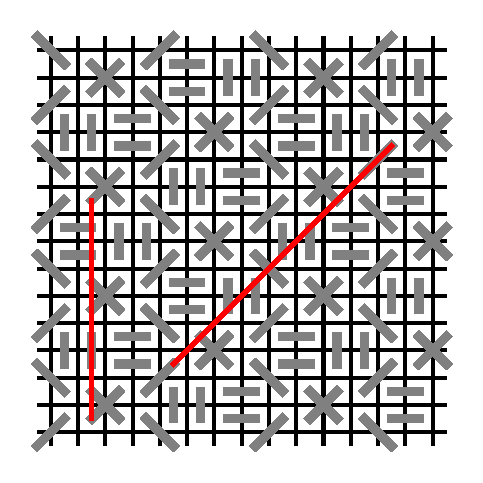
\includegraphics{m-n-9.eps}
    \caption{(m, n, 9)-jeu}
    \label{fig:m-n-9}
\end{figure}

%% sous-jeu
\begin{figure}[h]
    \centering
    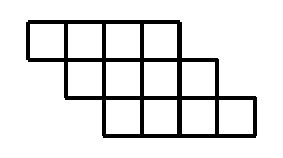
\includegraphics{m-n-8-little.eps}
    \caption{La grille du sous-jeu}
    \label{fig:sous-jeu}
\end{figure}

%% regle de sous-jeu
\begin{figure}[h]
    \centering
    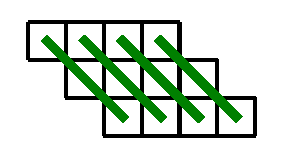
\includegraphics{8-rules1.eps}
    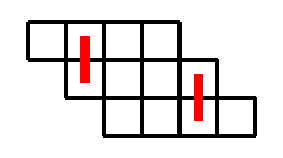
\includegraphics{8-rules2.eps}
    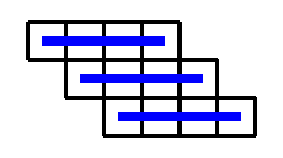
\includegraphics{8-rules3.eps}
    \caption{Les trois façons pour gagner le sous-jeu.}
    \label{fig:regle}
\end{figure}

%% m-n-8
\begin{figure}[h]
    \centering
    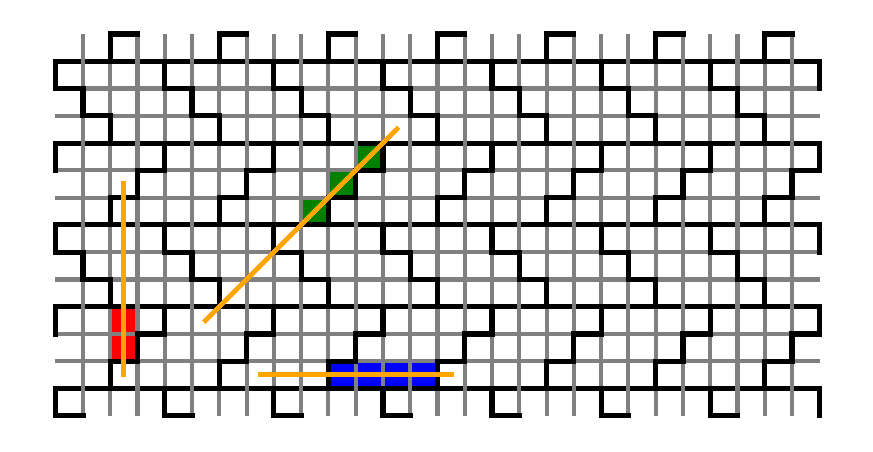
\includegraphics{8-sol.eps}
    \caption{(m, n, 8)-jeu:
    toutes les lignes de longueur 8 passent une des lignes gagantes du sous-jeu.}
    \label{fig:m-n-8}
\end{figure}
\end{document}
